% =====================================================================
%  Beamer Slides — Pipeline Summary
%  Zoobenthic Community Index Construction:
%  Methods, Data Flow, and Quality Assessment
% =====================================================================
\documentclass[aspectratio=169, 11pt]{beamer}

% ----- Theme & Colour ------------------------------------------------
\usetheme{Madrid}
\usecolortheme{default}
\definecolor{TRUblue}{HTML}{1565C0}
\definecolor{TRUgray}{HTML}{4A4A4A}
\setbeamercolor{structure}{fg=TRUblue}
\setbeamercolor{frametitle}{bg=TRUblue!10, fg=TRUblue}
\setbeamercolor{title}{fg=white, bg=TRUblue}
\setbeamercolor{block title}{bg=TRUblue, fg=white}
\setbeamercolor{block body}{bg=TRUblue!5}
\setbeamercolor{item}{fg=TRUblue}
\setbeamertemplate{navigation symbols}{}          % remove nav icons
\setbeamertemplate{footline}[frame number]        % simple page numbers

% ----- Packages -------------------------------------------------------
\usepackage[utf8]{inputenc}
\usepackage[T1]{fontenc}
\usepackage{graphicx}
\usepackage{booktabs}
\usepackage{amsmath, amssymb}
\usepackage{caption}
\usepackage{subcaption}          % side-by-side figures
\usepackage{xcolor}
\usepackage{hyperref}
\usepackage{adjustbox}           % rescale wide tables

% ----- Convenience Macros ---------------------------------------------
\newcommand{\hl}[1]{\textcolor{TRUblue}{\textbf{#1}}}
\newcommand{\figpath}{figures}   % <-- change to your figure folder
\newcommand{\code}[1]{\texttt{\small #1}}
\newcommand{\mat}[1]{\mathbf{#1}}
\newcommand{\R}{\mathbb{R}}
\newcommand{\PS}{\mathrm{PS}}
\newcommand{\ZCI}{\mathrm{ZCI}}
\newcommand{\BC}{\mathrm{BC}}

% ----- Title Info -----------------------------------------------------
\title[ZCI Pipeline Summary]{
    Steps in Computational Pipeline for
    Detection of Ecological Thresholds
}
\subtitle{Computational Pipeline Summary}
\author{Gu Feng}
\institute{Thompson Rivers University}
\date{March 5, 2026}

% =====================================================================
\begin{document}

% ----- Title Slide ----------------------------------------------------
\begin{frame}
  \titlepage
\end{frame}

% ----- Outline --------------------------------------------------------
\begin{frame}{Outline}
  \tableofcontents
\end{frame}

% =====================================================================
\section{Overview}
% =====================================================================

\begin{frame}{Core Computation Target}
  \begin{block}{Goal}
    Construct a \hl{Zoobenthic Community Index (ZCI)} that quantifies
    benthic community condition along a sediment-contamination gradient
    in the SCDRS corridor, and detect \hl{ecological thresholds} in such
    relationships.
  \end{block}

  \vspace{0.5em}
\end{frame}


\begin{frame}{Recall the expected visualizatoin of ZCI vs.\ Pollution Score}
    \begin{figure}
    \centering
    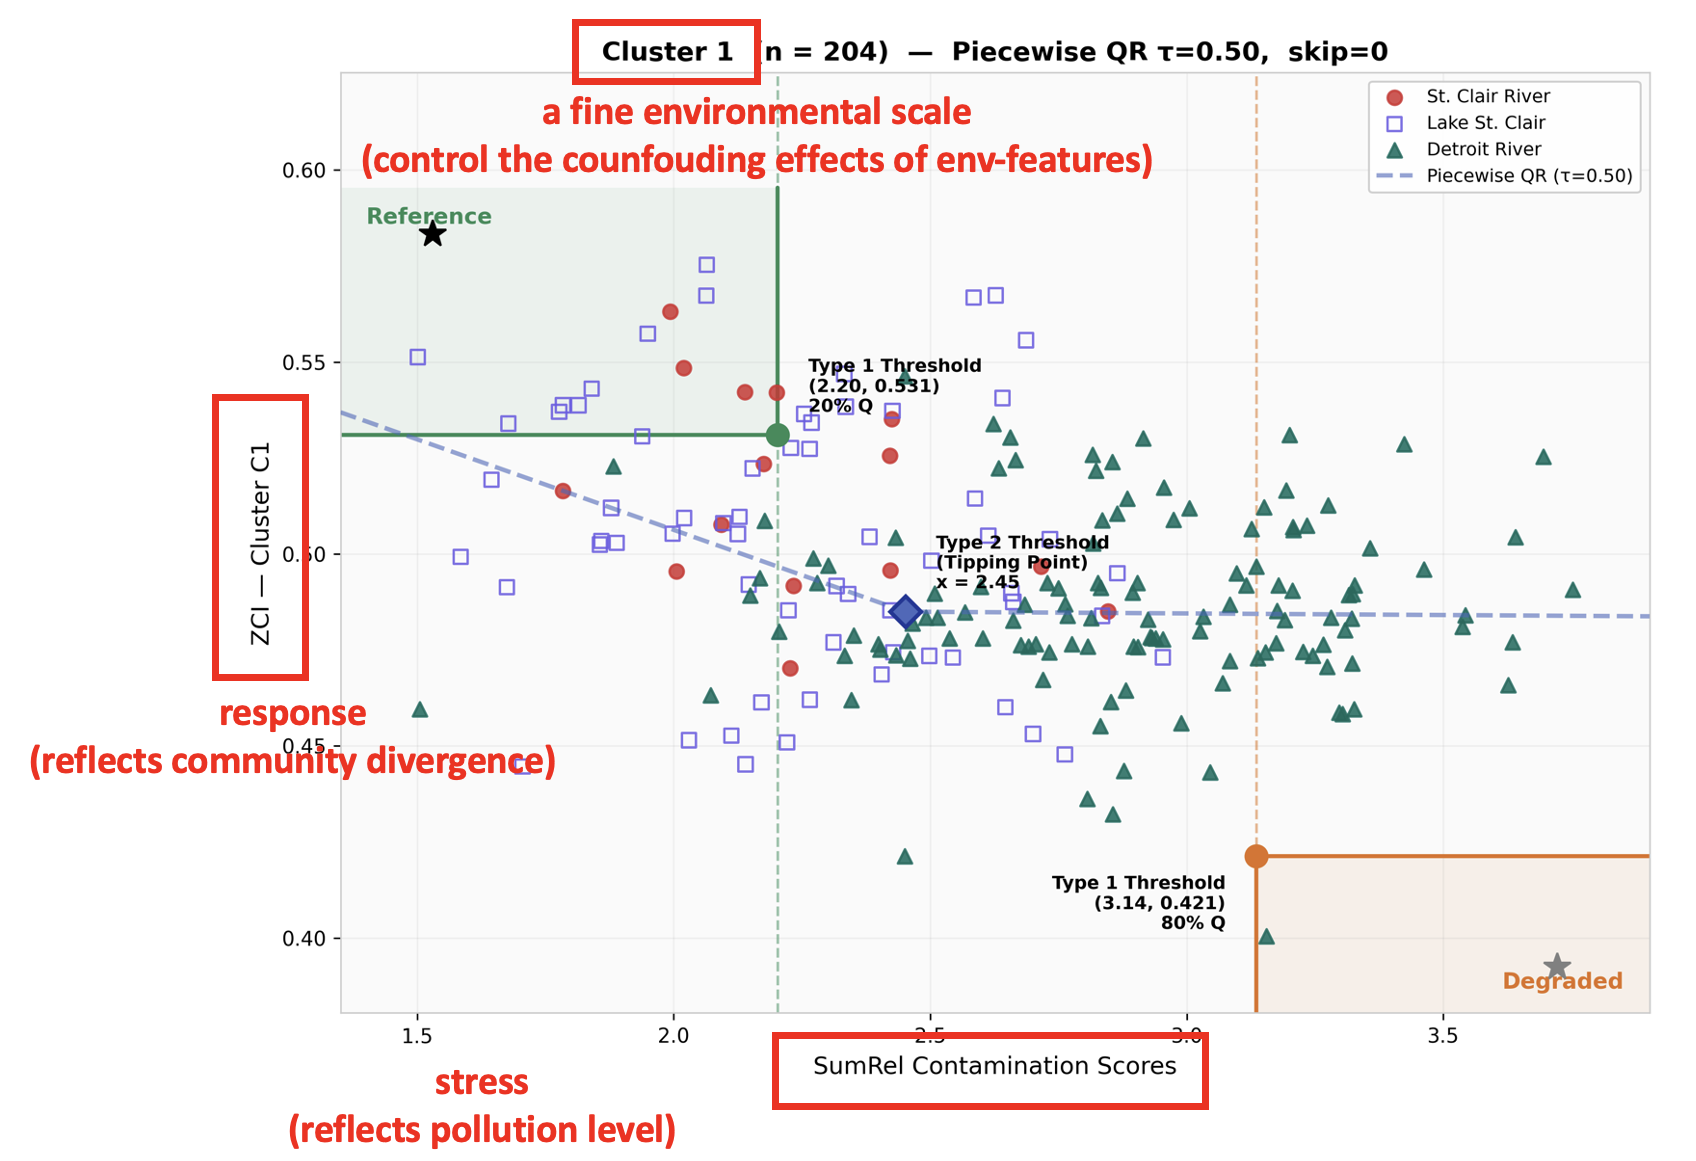
\includegraphics[width=0.6\textwidth]{images/three_key_questions2.png}
    \caption{ZCI vs.\ Pollution Score (Stage~5 piecewise quantile regression,
    still under development)}
    \end{figure}
  \vspace{0.5em}
\end{frame}


\begin{frame}{The tone behind the computational stages}
    \begin{block}{Goal}
    The computation work is very \hl{open} now, we can update many steps and integrate extensions,
    meanwhile keeping the \hl{integrity} of the current framework and results.
    \end{block}
    
\end{frame}


\begin{frame}{The framework to introduce each computation stage}
    \begin{enumerate}
        \item \textbf{Input data} --- what specific data blocks and columns are used in this stage
        \item \textbf{*Specific operation} --- transformation, model, normalization etc.
        \item \textbf{Outputs} --- what results, artifacts are remained
        \item \textbf{Potential issues and improvements to apply}
    \end{enumerate}
\end{frame}


\begin{frame}{The summary of all computation stages}
    \begin{figure}
    \centering
    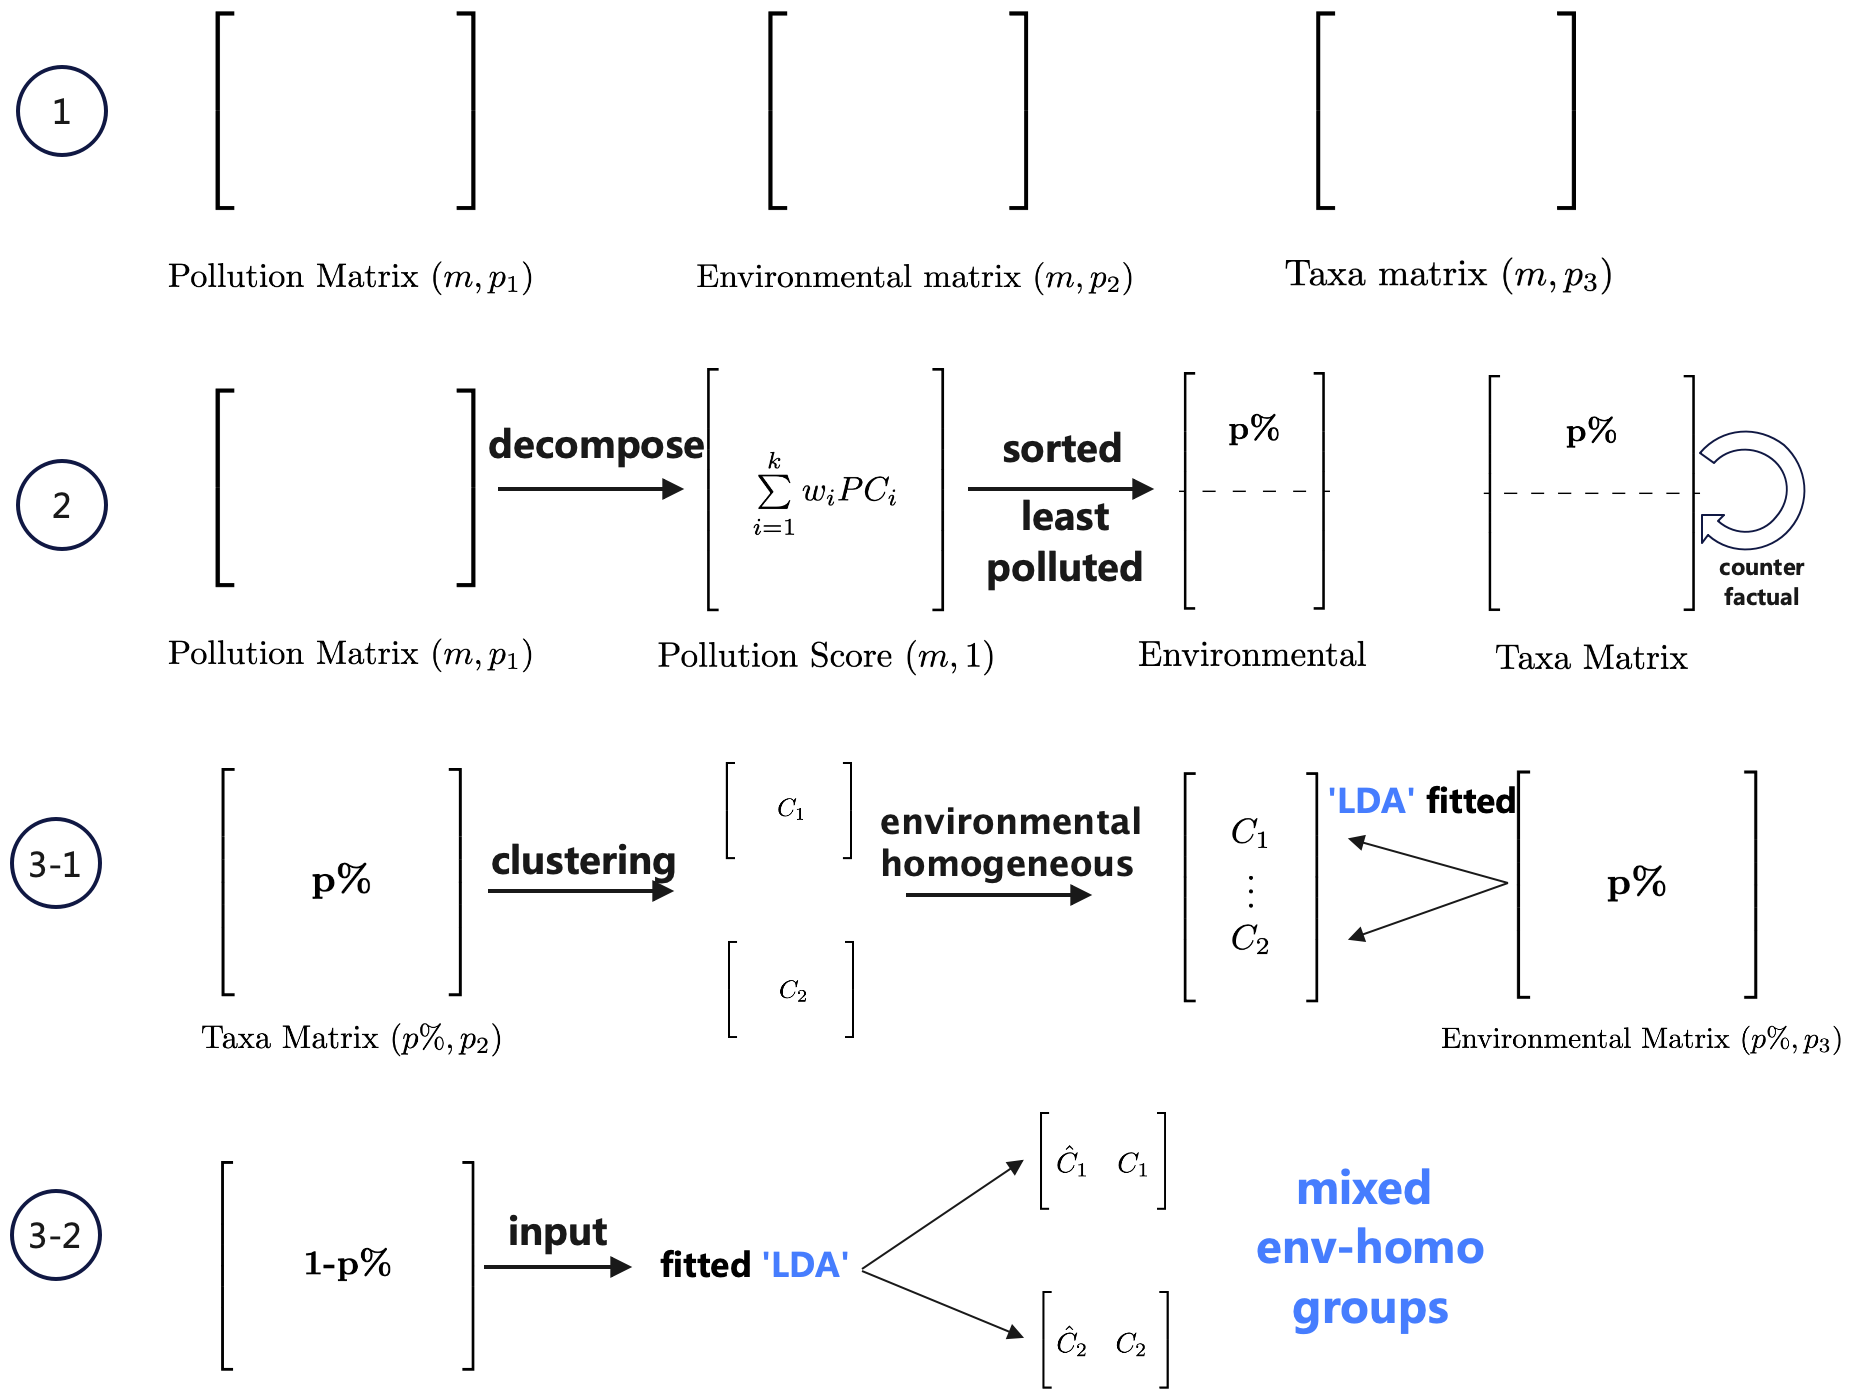
\includegraphics[width=0.65\textwidth]{images/overview_computation_stage0_to_3.png}
    \end{figure}
\end{frame}


\begin{frame}{The summary of all computation stages}
    \begin{figure}
    \centering
    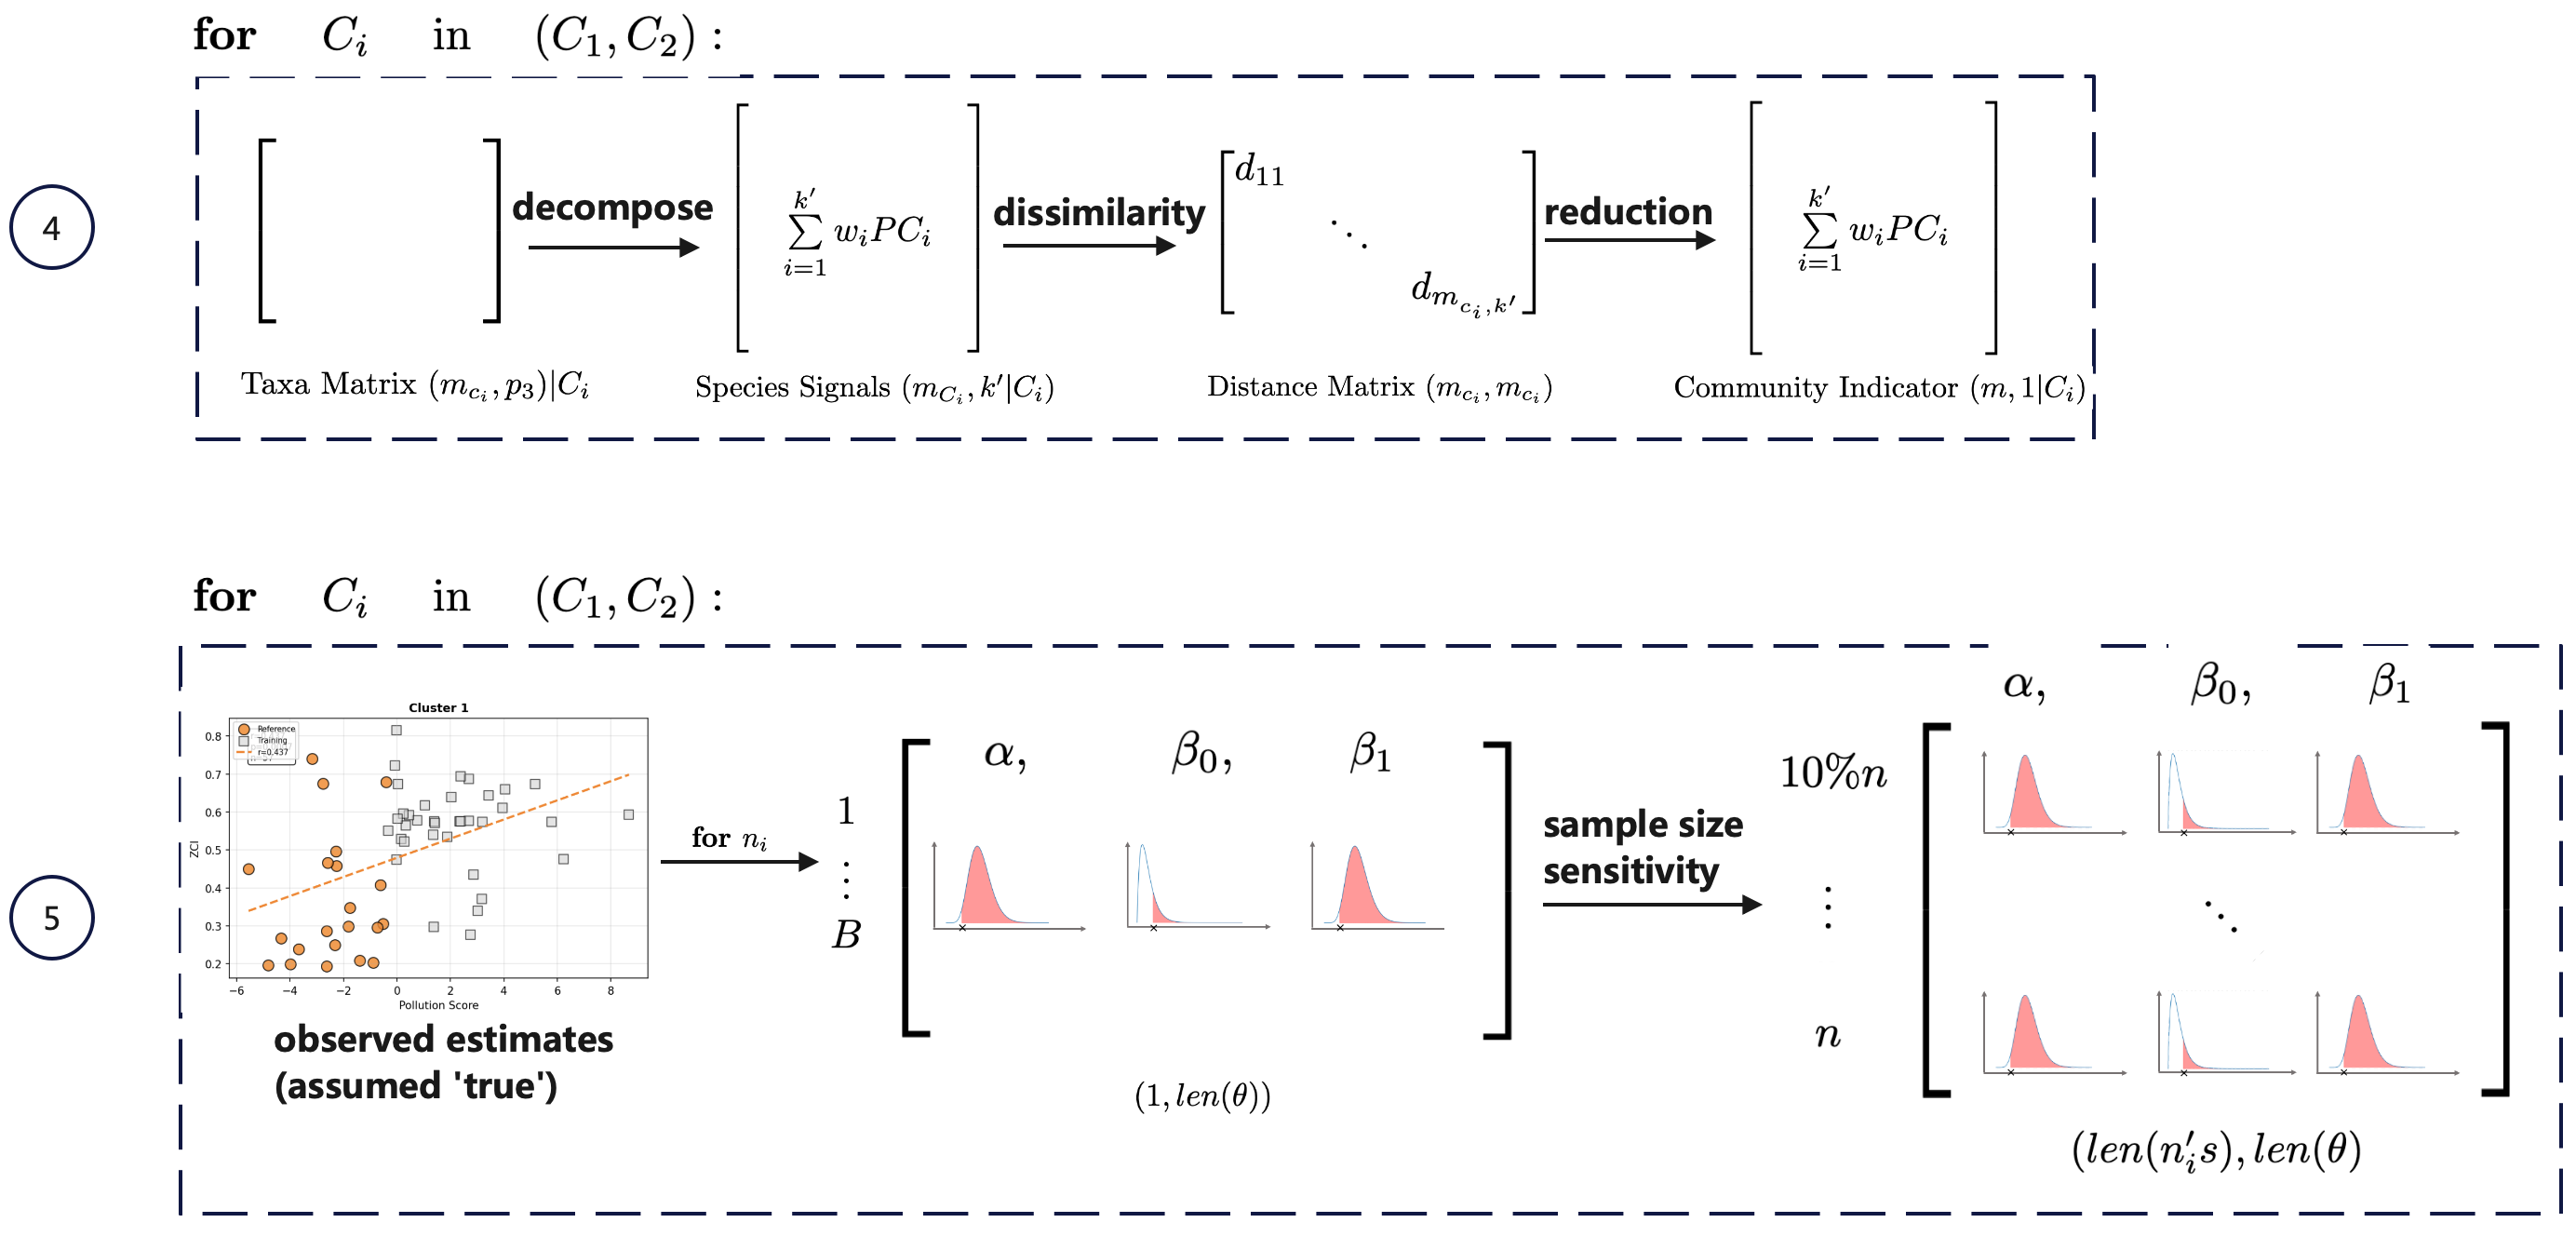
\includegraphics[width=0.7\textwidth]{images/overview_computation_stage4_to_5.png}
    \end{figure}
\end{frame}

\section{Stage 1 --- Pollution PCA}
% ---------------------------------------------------------------------
\begin{frame}{Stage 1: Pollution PCA --- Overview}
  \begin{center}
    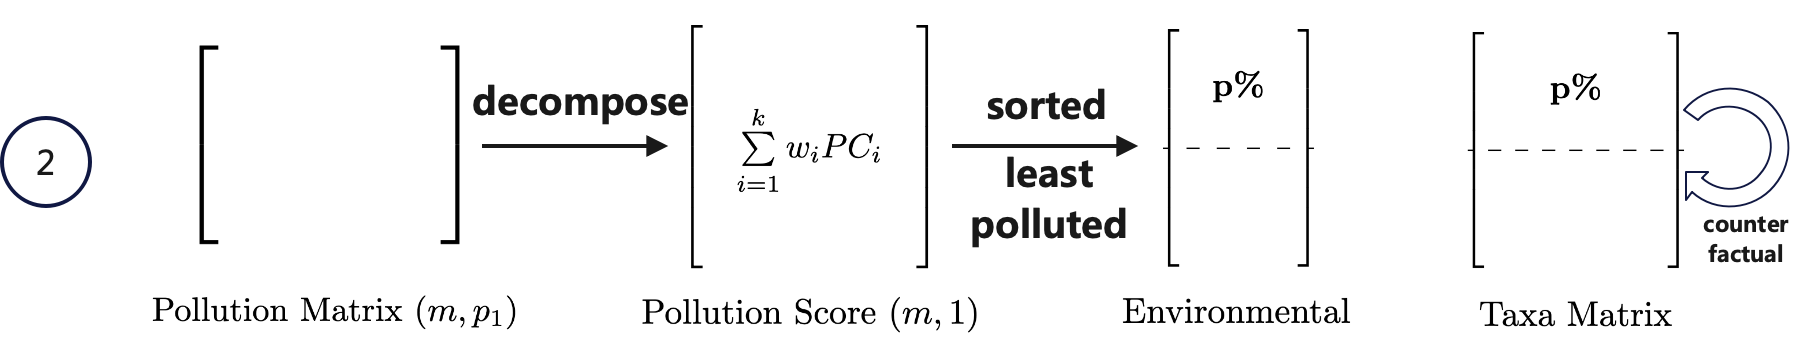
\includegraphics[width=0.75\textwidth]{images/overview_computation_stage1.png}
  \end{center}
\end{frame}

% ---------------------------------------------------------------------
\begin{frame}{Stage 1: Pollution PCA --- Input, Computation \& Output}
  \textbf{Input:} Chemical matrix $\mat{C}\in\R^{n\times 16}$ (16 sediment variables)

  \vspace{0.4em}
  \textbf{Computation:}
  \begin{enumerate}\small
    \item \textbf{Log$_2$ transform:}\;
          $\tilde{c}_{ij} = \log_2(1 + c_{ij})$
    \item \textbf{PCA} on $\tilde{\mat{C}}$ (centred, \emph{not} unit-scaled, $k{=}5$)
          \begin{itemize}\footnotesize
            \item Scaled loadings: $L_{jm} = v_{jm}\sqrt{\lambda_m}$
            \item Min--max scores: $s_{im}^{*} = \frac{s_{im} - \min}{\max - \min}$
          \end{itemize}
    \item \textbf{Composite score:}\;
          $s_i = \sum_{m=1}^{k} s_{im}^{*}$
  \end{enumerate}

  \vspace{0.3em}
  \textbf{Output:}
  {PC1--PC5, Pollution\_Score}
\end{frame}

% ---------------------------------------------------------------------
\begin{frame}{Stage 1: Design Notes \& Potential Issues}
  \begin{block}{Design Choice}
    PCA on log-transformed data \emph{without} unit-variance scaling
    $\Rightarrow$ high-variance contaminants dominate leading PCs.\\
    \smallskip
    \emph{Deliberate:} preserves natural scale differences among pollutants.
  \end{block}

  \vspace{0.4em}
  \begin{alertblock}{Potential Issues}
    \begin{itemize}\small
      \item No unit scaling --- pollution score weighted toward
            high-variance contaminants; should be noted explicitly
      \item Equal-weight PC summation ($w_m{=}1$) --- alternative
            weighting (e.g.\ by explained variance) not explored
      \item Min--max rescaling sensitive to outliers
    \end{itemize}
  \end{alertblock}
\end{frame}

% =====================================================================
\section{Stage 2 --- Taxa Assemblage Clustering}
% =====================================================================

% ---------------------------------------------------------------------
\begin{frame}{Stage 2: Taxa Assemblage Clustering --- Overview}
  \begin{center}
    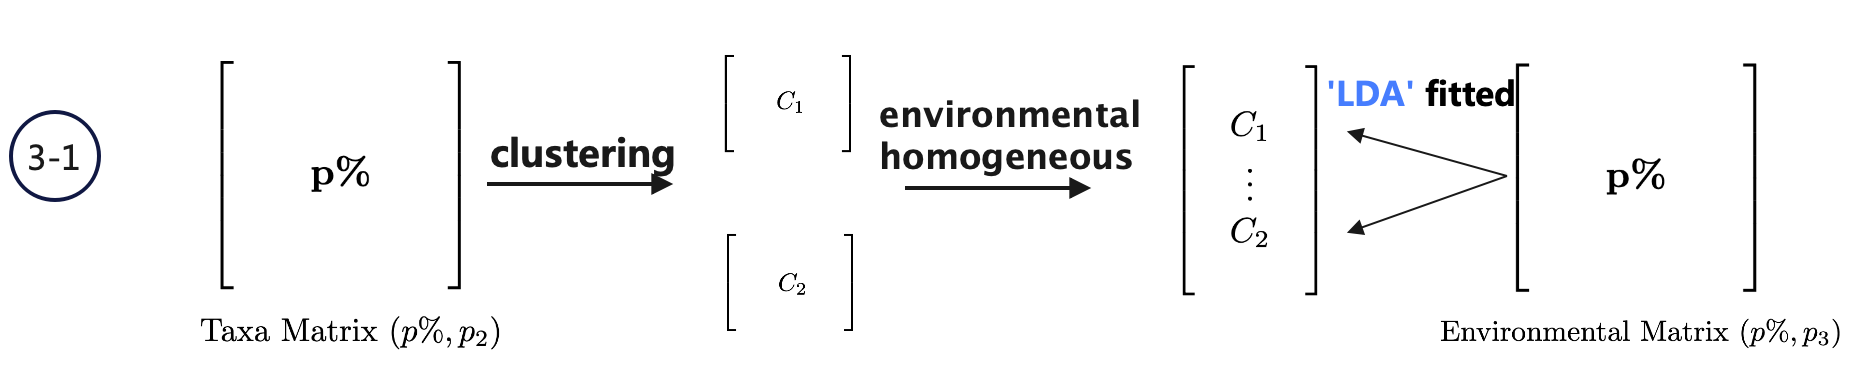
\includegraphics[width=0.75\textwidth]{images/overview_computation_stage2.png}
  \end{center}
\end{frame}

% ---------------------------------------------------------------------
\begin{frame}{Stage 2: Input, Computation \& Output}
  \textbf{Input:}
  \begin{itemize}\small
    \item Taxa block $\mat{O}\in\R^{n\times 16}$ (octave scale)
    \item Pollution Score $\mathbf{s}$ from Stage~1
  \end{itemize}

  \vspace{0.3em}
  \textbf{Computation:}
  \begin{enumerate}\small
    \item \textbf{Reference-site selection} --- bottom 20\% of pollution scores:
          $\;\mathcal{R} = \bigl\{ i : s_i \le s_{(\lfloor 0.20\,n \rfloor)} \bigr\}$
    \item \textbf{Taxa transform} --- octave values used as-is (default)
    \item \textbf{Ward's hierarchical clustering} on $\mat{O}_{\mathcal{R}}$,
          Euclidean distance, $K{=}3$ initial clusters:
          \[
            d_{\mathrm{merge}}(A,B) =
            \sqrt{\tfrac{2|A||B|}{|A|+|B|}}\;\|\bar{\mathbf{o}}_A - \bar{\mathbf{o}}_B\|
          \]
  \end{enumerate}

  \vspace{0.3em}
  \textbf{Output:} \code{02\_updated\_data.xlsx} --- \code{Cluster} labels for reference sites;
  non-reference sites remain \code{NaN}
\end{frame}

% ---------------------------------------------------------------------
\begin{frame}{Stage 2: Design Notes \& Potential Issues}
  \begin{block}{Design Choice}
    Ward's linkage minimises within-cluster variance ---
    favours compact, spherical clusters in octave space.
    The 20\% reference threshold is a \emph{subjective} cut-off.
  \end{block}

  \vspace{0.4em}
  \begin{alertblock}{Potential Issues}
    \begin{itemize}\small
      \item \textbf{Reference threshold sensitivity} --- the 20\% cut-off
            is arbitrary; varying it changes which sites are ``reference''
      \item \textbf{Number of clusters $K$} --- chosen by dendrogram
            inspection, not by a formal index (e.g.\ silhouette, gap statistic)
      \item \textbf{Octave-space distances} --- Ward's uses Euclidean distance
            on octave values; alternatives such as Bray--Curtis are not applicable
            with Ward's linkage
      \item Small clusters may be artefacts ($\Rightarrow$ handled by hindsight merge)
    \end{itemize}
  \end{alertblock}
\end{frame}


% =====================================================================
\section{Hindsight Relabel \& ANOVA}
% =====================================================================

% ---------------------------------------------------------------------
\begin{frame}{Hindsight \& ANOVA --- Overview}
  \begin{center}
    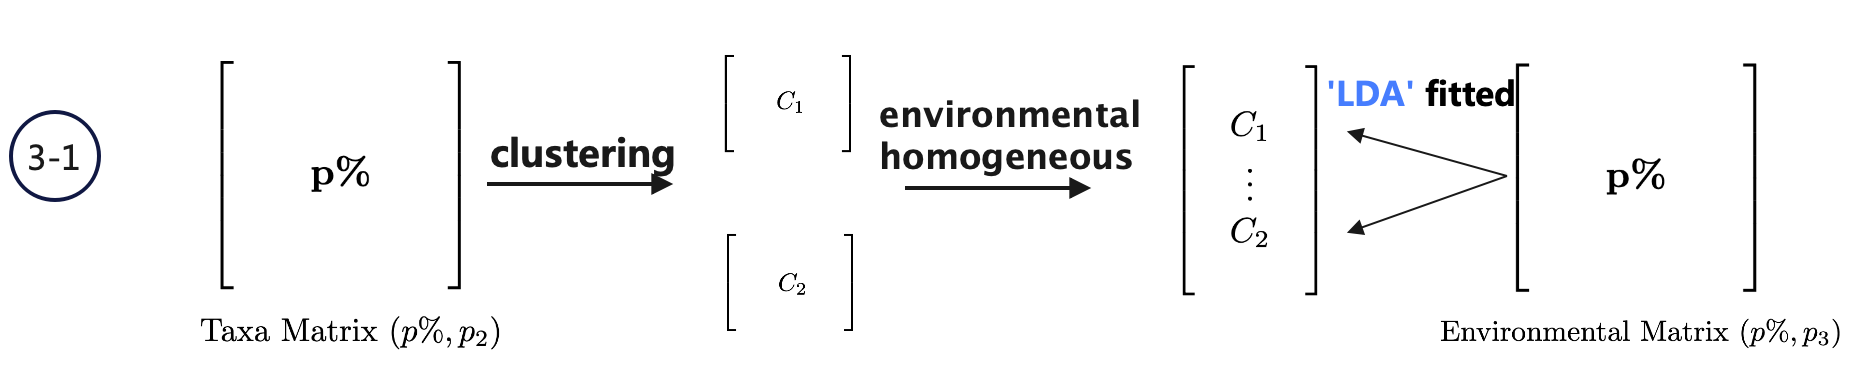
\includegraphics[width=0.75\textwidth]{images/overview_computation_stage2.png}
  \end{center}
  {\small\centering Hindsight relabelling and ANOVA validation operate on Stage~2 outputs.\par}
\end{frame}

% ---------------------------------------------------------------------
\begin{frame}{Hindsight: Input, Computation \& Output}
  \textbf{Input:} Stage~2 cluster labels + environmental \& taxa data (reference sites)

  \vspace{0.3em}
  \textbf{Computation:}
  \begin{enumerate}\small
    \item \textbf{Cluster relabelling} --- merge small clusters
          (e.g.\ $\{3 \to 1\}$) $\Rightarrow$ $K{=}2$ habitat groups
    \item \textbf{One-way ANOVA} per environmental variable \& taxon:
          \[
            F = \frac{\mathrm{SS}_{\text{btw}} / (K{-}1)}
                     {\mathrm{SS}_{\text{wth}} / (n_{\text{ref}}{-}K)}
          \]
          Optional pre-transforms: \code{none} | \code{log} | \code{boxcox}
  \end{enumerate}

  \vspace{0.3em}
  \textbf{Output:} \code{anova\_env.xlsx}, \code{anova\_taxa.xlsx},
  \code{cluster\_panel.png},\\
  \code{02\_hindsight\_updated\_data.xlsx}
\end{frame}

% ---------------------------------------------------------------------
\begin{frame}{Hindsight: Design Notes \& Potential Issues}
  \begin{block}{Role}
    ANOVA is \emph{supportive} --- it validates that habitat groups are
    ecologically distinct. It does \textbf{not} feed the ZCI computation.
  \end{block}

  \vspace{0.4em}
  \begin{alertblock}{Assumption Gap}
    \begin{itemize}\small
      \item No \textbf{Shapiro--Wilk} test for within-group normality
      \item No \textbf{Levene / Brown--Forsythe} test for equal variances
      \item No Q--Q plots or residual diagnostics generated
      \item \textbf{Recommend:} add assumption checks; use Welch's ANOVA
            or Kruskal--Wallis $H$ when assumptions fail;
            report effect sizes ($\eta^2$)
    \end{itemize}
  \end{alertblock}
\end{frame}


% =====================================================================
\section{Stage 3 --- LDA Classification}
% =====================================================================

% ---------------------------------------------------------------------
\begin{frame}{Stage 3: LDA Habitat Classification --- Overview}
  \begin{center}
    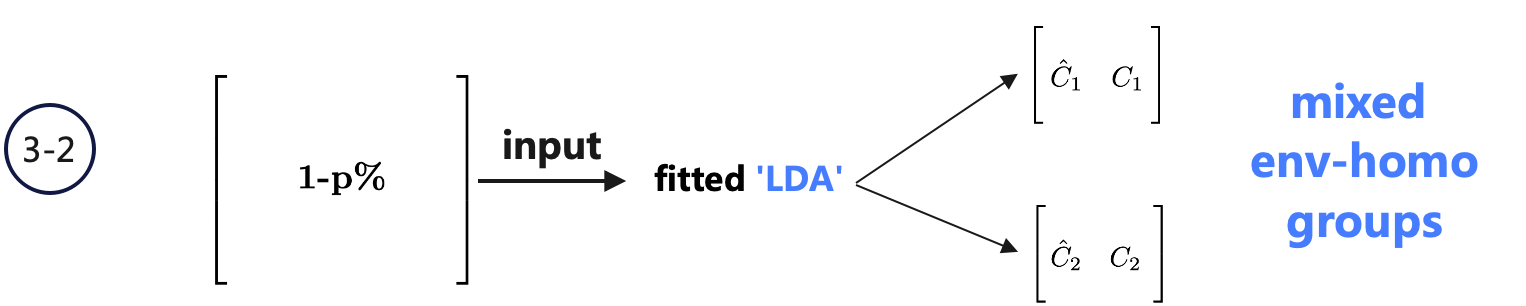
\includegraphics[width=0.75\textwidth]{images/overview_computation_stage3.png}
  \end{center}
\end{frame}

% ---------------------------------------------------------------------
\begin{frame}{Stage 3: Input, Computation \& Output}
  \textbf{Input:}
  \begin{itemize}\small
    \item Environmental matrix $\mat{E}_{\mathcal{R}}$ ($q{=}5$ variables:
          Depth, DO, Temperature, MPS, LOI)
    \item Cluster labels $\mathbf{g}_{\mathcal{R}}$ from hindsight artifact
    \item Pollution Score $\mathbf{s}$ (for reference-site identification)
  \end{itemize}

  \vspace{0.3em}
  \textbf{Computation:}
  \begin{enumerate}\small
    \item \textbf{$z$-score standardisation} on reference sites:
          $e_{ij}^{*} = (e_{ij} - \bar{e}_j)/\sigma_j$
    \item \textbf{LDA fitting} --- maximise between/within-class variance:
          $\mathrm{LD}_m = \mathbf{w}_m^{\!\top}\mathbf{e}^{*}$
    \item \textbf{Wilks' $\Lambda$} drop-one variable importance +
          Bartlett's $\chi^2$ overall test
    \item \textbf{Monte Carlo CV} --- 1\,000 stratified 80/20 splits
    \item \textbf{Predict} all non-reference sites $\Rightarrow$ habitat labels
  \end{enumerate}

  \vspace{0.3em}
  \textbf{Output:} \code{03\_updated\_data.xlsx} ---
  \code{Predicted\_Cluster}, \code{Is\_Reference}, LD coordinates, class probabilities
\end{frame}

% ---------------------------------------------------------------------
\begin{frame}{Stage 3: Design Notes \& Potential Issues}
  \begin{block}{Design Choice}
    LDA assumes multivariate normality and equal covariance matrices.
    Wilks' $\Lambda$ quantifies each variable's discriminatory contribution.
  \end{block}

  \vspace{0.4em}
  \begin{alertblock}{Potential Issues}
    \begin{itemize}\small
      \item \textbf{CV data leakage} --- \code{StandardScaler} fitted
            \emph{globally before} CV splits; test folds have indirect
            knowledge of training means/variances $\Rightarrow$ CV accuracy
            slightly optimistic
      \item \textbf{Fix:} refit scaler inside each CV fold
      \item \textbf{Small sample size} --- with $K{=}2$ and $|\mathcal{R}|$
            reference sites, LDA stability depends on adequate per-class $n$
      \item \textbf{Multivariate normality} not formally tested
    \end{itemize}
  \end{alertblock}
\end{frame}


% =====================================================================
\section{Stage 4 --- Bray--Curtis NMDS \& ZCI}
% =====================================================================

% ---------------------------------------------------------------------
\begin{frame}{Stage 4: Bray--Curtis NMDS \& ZCI --- Overview}
  \begin{center}
    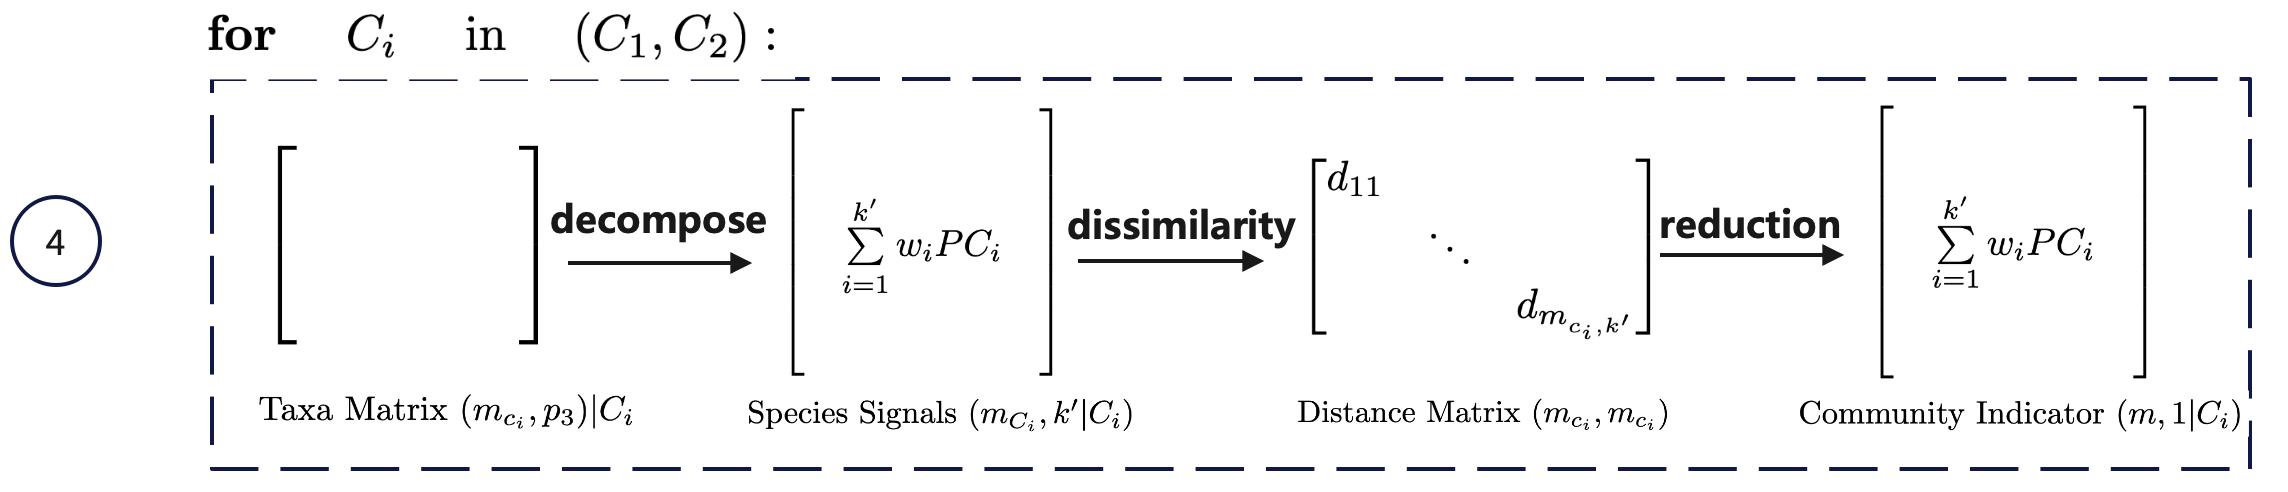
\includegraphics[width=0.75\textwidth]{images/overview_computation_stage4.png}
  \end{center}
\end{frame}

% ---------------------------------------------------------------------
\begin{frame}{Stage 4: Input, Computation \& Output}
  \textbf{Input:} Taxa $\mat{O}$ (octave), Pollution Score $\mathbf{s}$,
  Predicted Cluster $\mathbf{g}$

  \vspace{0.3em}
  \textbf{Computation (per cluster):}
  \begin{enumerate}\small
    \item \textbf{Octave $\to$ relative abundance:}
          $\hat{p}_{ij} = \max(0,\; 2^{o_{ij}} - 0.0625)$, row-normalise
    \item \textbf{Endpoint construction:} average the $n_{\text{ep}}$
          cleanest / most degraded sites $\Rightarrow$ synthetic reference
          \& degraded centroids
    \item \textbf{Bray--Curtis dissimilarity} (full pairwise matrix $\mat{D}$):
          $d_{\BC}(i,i') = \frac{\sum_j |p_{ij} - p_{i'j}|}{\sum_j (p_{ij} + p_{i'j})}$
    \item \textbf{Iterative NMDS} --- 3-pass SMACOF into $\R^2$; minimise stress
    \item \textbf{PCA rotation + axis flip} (NMDS1 $\leftarrow -$NMDS1 if $r > 0$)
    \item \textbf{Weighted-average species scores:}
          $\mathrm{WA}_j = \sum_i p_{ij}\mathbf{x}_i / \sum_i p_{ij}$
    \item \textbf{ZCI (BC-Direct):}
          $z_i = \frac{d_{\BC}(i, \mathcal{E}_{\text{deg}})}
                      {d_{\BC}(i, \mathcal{E}_{\text{ref}}) + d_{\BC}(i, \mathcal{E}_{\text{deg}})}$
  \end{enumerate}

  \vspace{0.2em}
  \textbf{Output:} \code{04\_updated\_data.xlsx} --- NMDS1, NMDS2, ZCI, ZCI\_Method
\end{frame}

% ---------------------------------------------------------------------
\begin{frame}{Stage 4: Where Bray--Curtis Is Applied (Twice)}
  Bray--Curtis enters at \textbf{two distinct points}:

  \vspace{0.3em}
  \begin{columns}[T]
    \begin{column}{0.48\textwidth}
      \begin{block}{1.\ For NMDS Ordination}
        Full pairwise $\mat{D}$ among all cluster sites + 2 endpoints.\\
        $\mat{D}$ feeds the SMACOF algorithm $\Rightarrow$ 2-D embedding.\\
        \smallskip
        {\small Purpose: \emph{visualisation} of community structure.}
      \end{block}
    \end{column}
    \begin{column}{0.48\textwidth}
      \begin{block}{2.\ For BC-Direct ZCI}
        Each site vs.\ endpoint \emph{centroids} only.\\
        Operates directly on $\mat{P}$ --- \textbf{independent} of NMDS.\\
        \smallskip
        {\small Purpose: the \emph{actual} community condition index.}
      \end{block}
    \end{column}
  \end{columns}

  \vspace{0.5em}
  \begin{center}\small
  \begin{tabular}{ccc}
    \toprule
    Cluster & $n_{\text{ep}}$ & Method \\
    \midrule
    1 & 15 & BC-Direct \\
    2 & 3  & BC-Direct \\
    \bottomrule
  \end{tabular}
  \end{center}
\end{frame}

% ---------------------------------------------------------------------
\begin{frame}{Stage 4: Design Notes \& Potential Issues}
  \begin{alertblock}{Issues in Current Implementation}
    \begin{itemize}\small
      \item \textbf{NMDS axis flip is enforced, not discovered} ---
            NMDS1 is flipped so $r(\text{NMDS1}, \mathbf{s}) < 0$;
            the negative correlation is an \emph{artefact of convention},
            not evidence of a contamination gradient
      \item \textbf{Endpoint sensitivity} --- small $n_{\text{ep}}$
            (e.g.\ 3 for Cluster~2) makes the centroid sensitive to
            individual outlier sites; ZCI stability under varying
            $n_{\text{ep}}$ should be reported
      \item \textbf{NMDS stress} --- if stress $> 0.20$, the 2-D
            representation is unreliable; must be evaluated per cluster
      \item \textbf{Cluster-specific ZCI} --- computed separately
            within each habitat cluster; cross-cluster ZCI comparisons
            require caution (different endpoint communities)
      \item \textbf{ZCI uses BC-Direct (not NMDS coords)} --- more
            defensible but means NMDS serves only visualisation, not
            the index itself
    \end{itemize}
  \end{alertblock}
\end{frame}


% =====================================================================
\section{Stage 5 --- Piecewise Quantile Regression}
% =====================================================================

% ---------------------------------------------------------------------
\begin{frame}{Stage 5: Piecewise Quantile Regression --- Overview}
  \begin{center}
    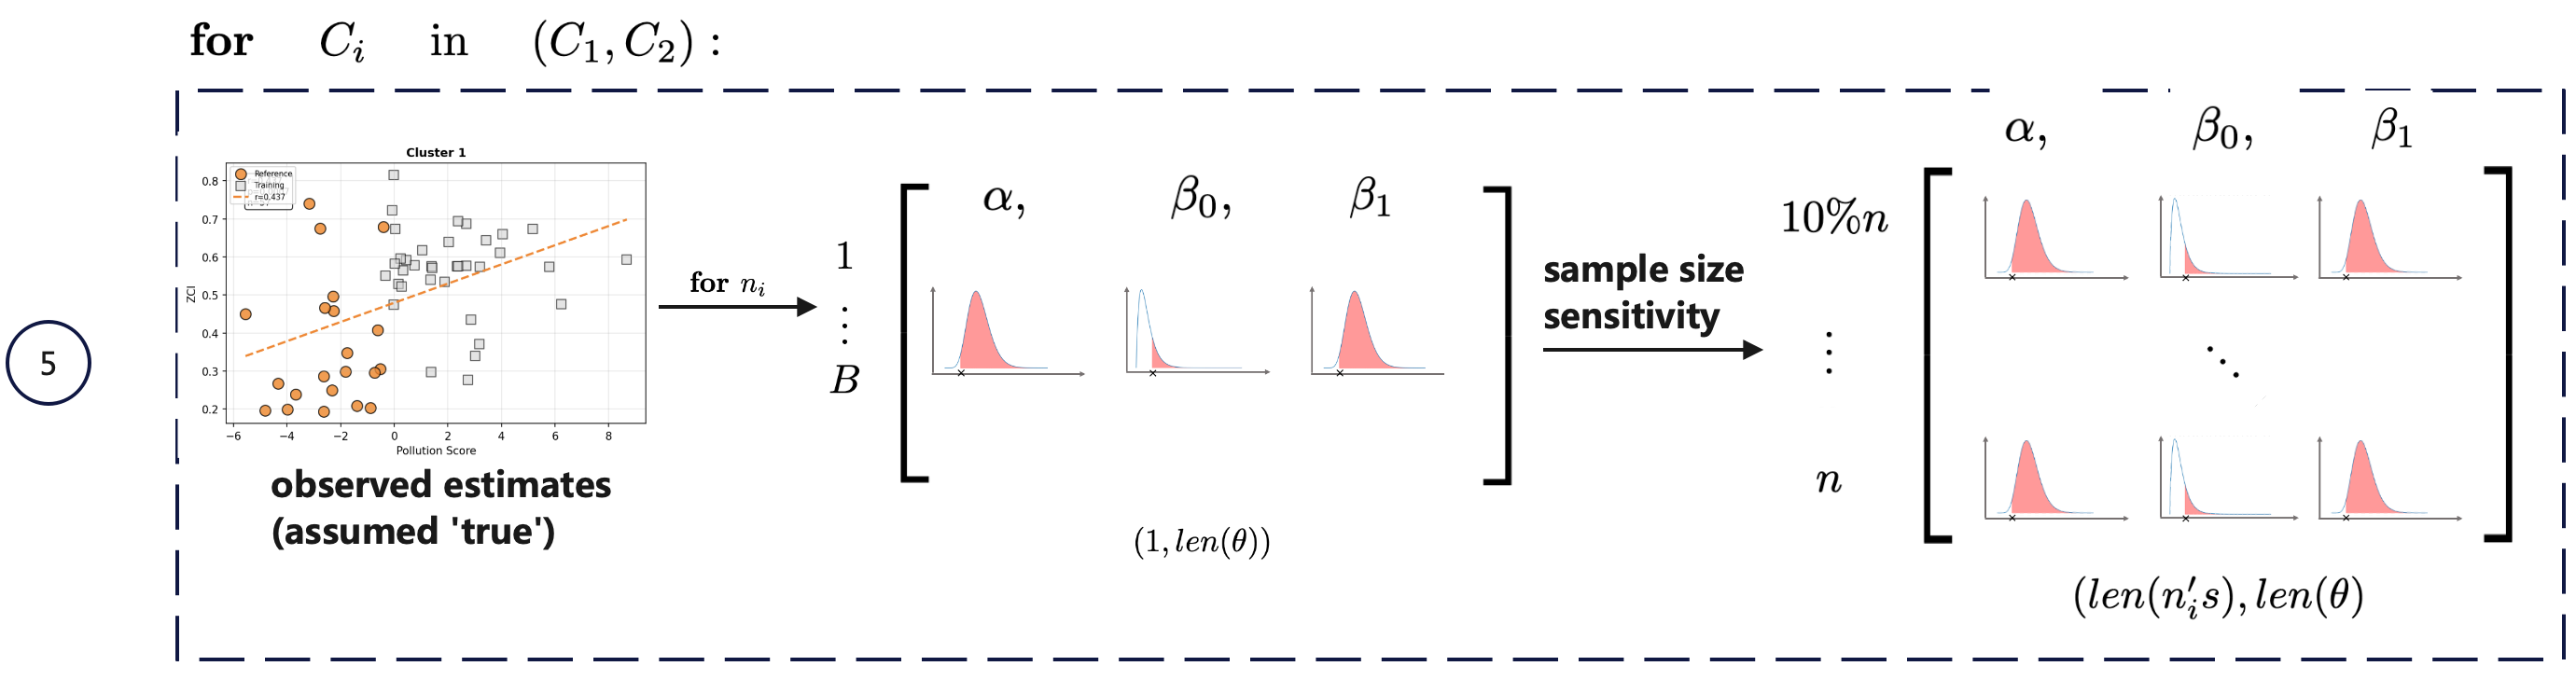
\includegraphics[width=0.75\textwidth]{images/overview_computation_stage5.png}
  \end{center}
\end{frame}

% ---------------------------------------------------------------------
\begin{frame}{Stage 5: Input, Computation \& Output}
  \textbf{Input:} Pollution Score $\mathbf{s}$ (S1),
  Predicted Cluster $\mathbf{g}$ (S3), ZCI $\mathbf{z}$ (S4)

  \vspace{0.3em}
  \textbf{Computation} (per cluster, $\tau \in \{0.10, 0.15, \dots, 0.90\}$):
  \begin{enumerate}\small
    \item \textbf{Piecewise linear quantile regression:}
          \[
            Q_\tau(\ZCI \mid \PS{=}x)
            = \beta_0 + \beta_1 x + \beta_2 (x - \psi)_+
          \]
    \item \textbf{Profile grid search} over candidate breakpoints $\psi$;
          LP sub-problem at each $\psi_c$
    \item \textbf{Wild bootstrap CI} (Feng, He \& Hu 2011) ---
          Mammen's two-point weights, $B{=}500$ replicates, 90\% CI
  \end{enumerate}

  \vspace{0.3em}
  \textbf{Output:} \code{05\_updated\_data.xlsx} ---
  breakpoint $\hat\psi$, slope coefficients, CI bounds per $\tau$

  \vspace{0.2em}
  {\small\emph{Note:} Stage~5 is currently commented out in the corridor-wide runner;
  active in the Detroit River runner.}
\end{frame}

% ---------------------------------------------------------------------
\begin{frame}{Stage 5: Design Notes \& Potential Issues}
  \begin{block}{Design Choice}
    Piecewise quantile regression detects \emph{threshold breakpoints}
    in the ZCI--Pollution relationship at multiple quantile levels,
    capturing heterogeneous community responses.
  \end{block}

  \vspace{0.4em}
  \begin{alertblock}{Potential Issues}
    \begin{itemize}\small
      \item \textbf{Grid resolution} for $\psi$ --- coarse grid may miss
            the optimal breakpoint; finer grid increases computation
      \item \textbf{Bootstrap $B$} --- 500 replicates adequate for 90\% CI
            but may be insufficient for 95\% CI; consider $B \ge 1000$
      \item \textbf{Edge effects} --- grid spans 10th--90th percentile;
            breakpoints near extremes are not detectable
      \item \textbf{Single breakpoint model} --- only one hinge; multiple
            thresholds would require spline or multi-breakpoint extensions
    \end{itemize}
  \end{alertblock}
\end{frame}


% =====================================================================
\section{RDA Validation}
% =====================================================================

\begin{frame}{Stage RDA: Redundancy Analysis (Complementary)}
  \textbf{Purpose:} Quantify how much taxa variation is explained by environmental predictors.

  \vspace{0.3em}
  \begin{enumerate}
    \item Multivariate OLS: $\hat{\mat{Y}} = \mat{X}_c\hat{\mat{B}}$
    \item PCA on fitted values $\Rightarrow$ constrained eigenvalues
    \item Permutation tests (999 permutations):
  \end{enumerate}

  \vspace{0.3em}
  \begin{center}\small
  \begin{tabular}{lp{8cm}}
    \toprule
    Test & Null hypothesis \\
    \midrule
    Global   & No linear relationship between $\mat{Y}$ and $\mat{X}$ \\
    Per-axis & Individual RDA axis non-significant \\
    Per-term & Individual variable non-significant (Freedman--Lane) \\
    \bottomrule
  \end{tabular}
  \end{center}

  \vspace{0.3em}
  \textbf{Does not feed downstream stages} --- validation only.
\end{frame}

% =====================================================================
\section{Artifact Chain}
% =====================================================================

\begin{frame}{Stage-by-Stage Artifact Chain}
  \begin{center}\small
  \renewcommand{\arraystretch}{1.15}
  \begin{tabular}{l p{3.2cm} p{4.5cm} p{3.5cm}}
    \toprule
    Stage & Input & New Columns & Output \\
    \midrule
    S1 (PCA)    & Original workbook  & PC1--5, Pollution\_Score  & \code{01\_updated.xlsx} \\
    RDA         & Orig + S1          & \emph{None (figs/tables)} & \emph{No artifact} \\
    S2 (Clust.) & Orig + S1          & Cluster, Is\_Reference    & \code{02\_updated.xlsx} \\
    Hindsight   & S2 + Orig          & Relabelled Cluster        & \code{02\_hind.xlsx} \\
    S3 (LDA)    & Orig + S1 + Hind.  & Pred.\ Cluster, LD1      & \code{03\_updated.xlsx} \\
    S4 (NMDS)   & Orig + S1 + S3     & NMDS1/2, ZCI             & \code{04\_updated.xlsx} \\
    S5 (PQR)    & S1 + S3 + S4       & Model params             & \code{05\_updated.xlsx} \\
    \bottomrule
  \end{tabular}
  \end{center}
\end{frame}


% =====================================================================
\section{TITAN Integration}
% =====================================================================

% ---------------------------------------------------------------------
\begin{frame}{TITAN: How It Complements the Current Framework}
  \begin{columns}[T]
    \begin{column}{0.55\textwidth}
      \begin{block}{What TITAN Adds}
        A \hl{taxon-resolution layer} the pipeline currently lacks:
        \emph{which} taxa drive community shifts and at \emph{what}
        pollution level.
      \end{block}

      \vspace{0.3em}
      \textbf{Algorithm (per cluster):}
      \begin{enumerate}\footnotesize
        \item Binary partitions along the pollution gradient
        \item IndVal per taxon per split $\Rightarrow$ $z$-score vs.\ permutation null
        \item Change-point: $x_c^{*(j)} = \arg\max_{x_c} z_j(x_c)$
        \item Direction: $z^{-}$ (sensitive) vs.\ $z^{+}$ (tolerant)
        \item Bootstrap purity $\ge 0.95$ \& reliability $\ge 0.95$
        \item Community threshold: peak of $\mathrm{sum}(z^{\pm})$
      \end{enumerate}
    \end{column}
    \begin{column}{0.42\textwidth}
      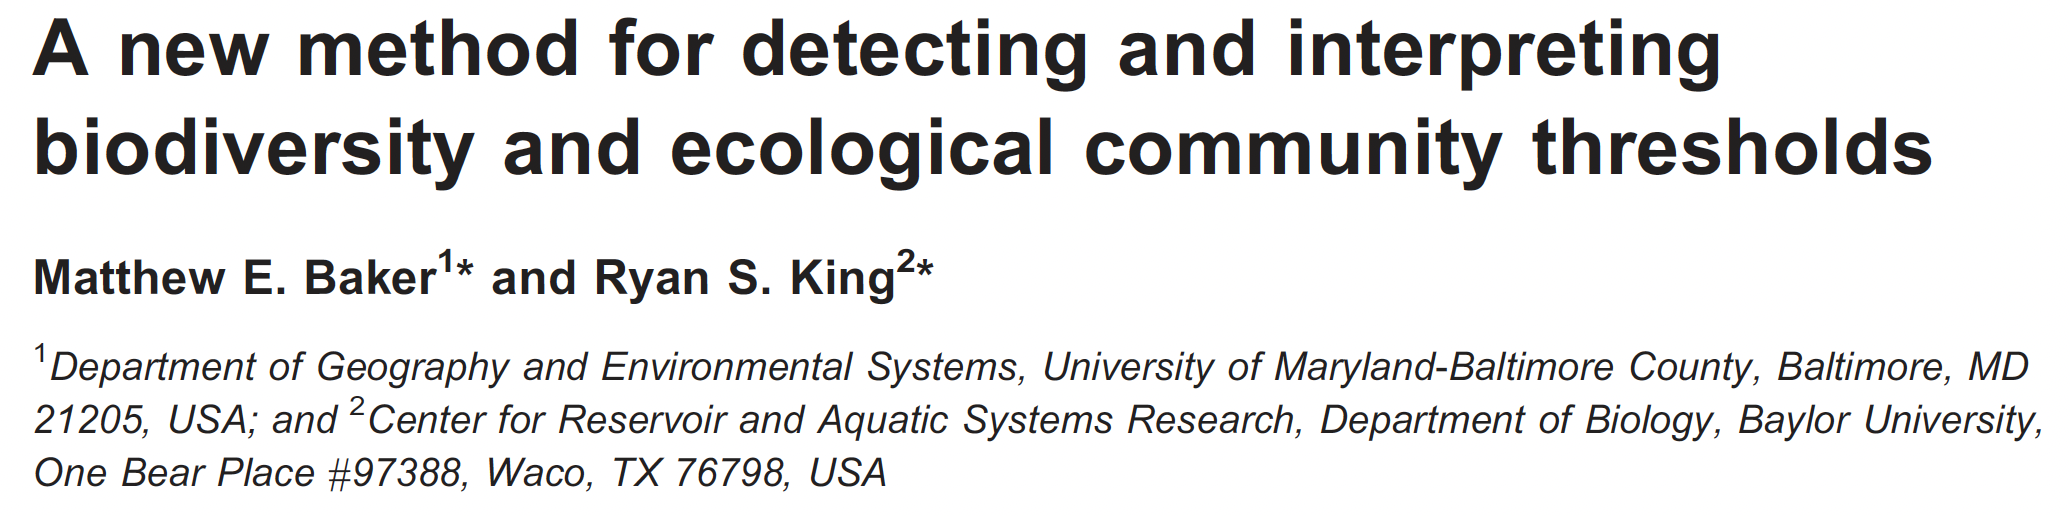
\includegraphics[width=\textwidth]{images/ref_TITAN.png}

      \vspace{0.3em}
      {\footnotesize\centering Reference: Baker \& King (2010)\par}
    \end{column}
  \end{columns}
\end{frame}

% ---------------------------------------------------------------------
\begin{frame}{TITAN: Integration Plan \& Key Questions}
  \textbf{Input from existing pipeline:}
  \begin{center}\small
  \begin{tabular}{lll}
    \toprule
    TITAN Input & Source & Stage \\
    \midrule
    Gradient $x$           & Pollution\_Score        & Stage~1 \\
    Taxa matrix $\mat{Y}$  & Relative abundance $\mat{P}$     & Octave inverse \\
    Cluster grouping       & Predicted\_Cluster      & Stage~3 \\
    \bottomrule
  \end{tabular}
  \end{center}

  \vspace{0.3em}
  \textbf{Key questions TITAN answers:}
  \begin{itemize}
    \item Does the 20\% reference threshold match an \hl{ecological change point}?
    \item Gradual taxon turnover or \hl{abrupt regime shift}?
    \item Independent comparison with Stage~5 piecewise-QR breakpoint $\hat\psi$
    \item Which individual taxa are responsible for the community shift?
  \end{itemize}

  \vspace{0.3em}
  \textbf{Execution:} R package \code{TITAN2} via \code{rpy2};
  overlay $\mathrm{sum}(z^{\pm})$ peaks as vertical lines on ZCI--Pollution plots
\end{frame}


% =====================================================================
\section{Recommendations}
% =====================================================================

\begin{frame}{Summary of Recommendations}
  \begin{enumerate}
    \item \hl{ANOVA assumptions}: add Shapiro--Wilk + Levene's tests;
          Welch/Kruskal--Wallis as robust alternatives
    \item \hl{LDA CV leakage}: move \code{StandardScaler} inside each fold
    \item \hl{NMDS axis-flip}: state explicitly that orientation is enforced
    \item \hl{Endpoint sensitivity}: report ZCI stability under varying $n_{\text{ep}}$
    \item \hl{PCA scaling}: note log-transformed but not unit-scaled
    \item \hl{TITAN}: embed per-cluster analysis after Stage~3;
          overlay thresholds on ZCI--Pollution plots
  \end{enumerate}
\end{frame}

% ----- Thank You / Questions -----------------------------------------
\begin{frame}{}
  \centering
  \vspace{2cm}
  {\Huge\color{TRUblue} Questions?}

  \vspace{1.5cm}
  {\large Gu Feng \quad|\quad Thompson Rivers University}
\end{frame}

\end{document}
